%===============================================================================
% DOCUMENT
%===============================================================================

%% Document class
\documentclass[a4paper,12pt]{scrreprt}

%% Include packages
\usepackage{packages}

\begin{document}

%% Include custom commands
\include{commands}

\pagenumbering{gobble}

%% Build cover
\definecolor{titlepagecolor}{RGB}{37,64,56}

%==========================================================================
% COLORED BAR ON THE LEFT SIDE
%==========================================================================

\backgroundsetup{
    scale=1,
    angle=0,
    opacity=1,
    contents={
        \begin{tikzpicture}[remember picture,overlay]
            \path [fill=titlepagecolor] (-10.5,-15) rectangle ++ (5,30);
            \node[color=white] at (-6.90,-11.5) {\bfseries {\fontsize{120}{60} \textsf{C}}};
            \node[color=titlepagecolor] at (-4.30,-11.5) {\bfseries {\fontsize{120}{60} \textsf{C}}};
        \end{tikzpicture}
    }
}

%==========================================================================
% COVER PAGE CONTENT
%==========================================================================

\title{\LARGE{Network Monitoring System}}

\author{
    Flávia Alexandra da Silva Araújo (A96587)\\ \quad
    Joshua David Amaral Moreira (A105684)\\ \quad
    Miguel Torres Carvalho (A95485)\\ \quad
}

%% Date
\date{\today}

%% Course
\newcommand{\Course}{Licenciatura em Engenharia Informática}

%% Department
\newcommand{\Department}{Escola de Engenharia}

%% UniName
\newcommand{\UniName}{Universidade do Minho}

%% UniPic
\newcommand{\UniPic}{
\includegraphics[width=120pt]{img/eeum.png}}

%% University
\newcommand{\University}{
    \begin{flushleft}
        \UniPic
    \end{flushleft}
    \textcolor{gray}{\small\textbf{\textsf{\UniName}}}\par
    \textcolor{gray!80!white}{\small{\textsf{\Department}}}\par
    \textcolor{gray!70!white}{\small{\textsf{\Course}}}
}

%% UC
\newcommand{\UC}{
    \begin{flushleft}
        \par\textcolor{titlepagecolor}{\Large\textbf{\textsf{Comunicações por Computador}}}
    \end{flushleft}
}

%% Project Phase
\newcommand{\SubTitle}{
    \begin{flushleft}
        \large\textbf{Trabalho Prático 2}
    \end{flushleft}
}

%% Group Info
\newcommand{\GroupInfo}{\par Grupo 10 - PL1}

%% GitHub Repo
\newcommand{\GitHubRepo}{\par\url{https://github.com/migueltc13/CC-tp2}}

%% School Year
\newcommand{\SchoolYear}{
    \par\small{\textsf{Ano Letivo de 2024/2025}}
}

%% Define new command to show title, author and date
\makeatletter
\let\Title\@title
\let\Author\@author
\let\Date\@date
\makeatother

%==========================================================================
% BEGIN COVER PAGE
%==========================================================================

%% Make cover page
\newcommand{\makecover}{

%% Removes page number on footer
\thispagestyle{empty}

%% No indentation
\setlength{\parindent}{0em}

%% Put Background defined on \backgroundsetup, in this page
\BgThispage

%% Changing geometry to prevent overlay with text
%% At the end of back cover, geometry is default with \restoregeometry
\newgeometry{top=4cm,left=6cm,right=2cm,bottom=2cm}

%% builds university info defined previously
\University
\vspace{1cm}
\UC
\SubTitle
\SchoolYear

\vspace*{4cm}
%% bigger space (i think its the default one) between paragraphs
\setlength{\parskip}{1em}

%% builds title info defined previously
\par\textbf{\textsf{\huge\Title}}
\vspace{1cm}
%% builds author(s) info defined previously
\par\Author

\vspace{0.5cm}

%% builds date info defined previously
\par\Date
\restoregeometry
\pagebreak

}

%==========================================================================
% END COVER PAGE
%==========================================================================

\makecover

%% Default geometry
\newgeometry{top=3cm,left=3cm,right=3cm,bottom=4cm}

%% Save default geometry
\savegeometry{default}

%% Load default geometry with:
% \loadgeometry{default}

%===============================================================================
% BEGIN ABSTRACT PAGE
%===============================================================================

\renewenvironment{abstract}
 {\par\noindent\textbf{\Large\abstractname}\par\bigskip}
 {}

\begin{flushleft}
\begin{abstract}
    \par
    No presente relatório, é apresentada a solução desenvolvida para a Unidade Curricular
    de \textbf{Comunicações por Computador}, como parte do projeto final do semestre - \textbf{\textit{Network Monitoring System}}.
    Este trabalho teve como objetivo projetar um sistema capaz de monitorizar e analisar o tráfego de rede entre um servidor
    central e vários agentes distribuídos, permitindo a recolha de métricas de desempenho e a execução de tarefas de monitorização.

    O sistema foi desenvolvido utilizando dois protocolos aplicacionais principais: \textbf{\textit{AlertFlow}}, destinado à gestão de alertas,
    e \textbf{\textit{NetTask}}, que assegura a comunicação robusta e confiável entre o servidor e os agentes. Foram implementadas funcionalidades
    de tolerância a falhas e adaptação a condições adversas, como alta latência e perda de pacotes, garantindo a integridade dos dados transmitidos.

    O trabalho foi concluído com a implementação e validação das principais funcionalidades do sistema, demonstrando a sua eficácia em ambientes
    de teste representativos. Este relatório documenta detalhadamente o \textit{design}, a implementação e os resultados obtidos.

    \par \textbf{Palavras-Chave}: \textit{Network Monitoring System}, \textit{AlertFlow}, \textit{NetTask}, \textit{Comunicações por Computador}.
\end{abstract}
\end{flushleft}

\pagebreak

%===============================================================================
% END ABSTRACT PAGE
%===============================================================================

%===============================================================================
% BEGIN INDEXES PAGES
%===============================================================================

%% Changes table of content name
\renewcommand{\contentsname}{Índice}
\renewcommand{\listfigurename}{Índice de Figuras}
\renewcommand{\listtablename}{Índice de Tabelas}
\renewcommand{\lstlistlistingname}{Índice de \textit{Snippets}}

\tableofcontents
\pagebreak

\listoffigures
\pagebreak

\listoftables
\pagebreak

\lstlistoflistings
\pagebreak

%===============================================================================
% END INDEXES PAGES
%===============================================================================

\pagenumbering{arabic}

%===============================================================================
% BEGIN ARQUITETURA DA SOLUÇÃO
%===============================================================================

\chapter{Arquitetura da Solução}

\textcolor{red}{
    Dúvida: o diagrama da arquitetura da solução deve ser
    mais geral ou mais específico à solução (python) desenvolvida?
}

%===============================================================================
% END ARQUITETURA DA SOLUÇÃO
%===============================================================================

%===============================================================================
% BEGIN ESPECIFICACÕES DOS PROTOCOLOS APLICACIONAIS
%===============================================================================

\chapter{Especificações dos Protocolos Aplicacionais}

\section{\textit{AlertFlow}}

\subsection{Formato de Mensagem}

\subsection{Diagrama de Sequência}

\begin{itemize}
    \item Normal
\end{itemize}

\clearpage

\section{\textit{NetTask}}

O protocolo \textit{NetTask} é essencial para a funcionalidade harmonizada do
\textbf{\textit{Network Monitoring System}}, sendo este usado para a maioria
das comunicações entre o servidor e os agentes, tais como, a primeira conexão de
um agente ao servidor, o envio de tarefas pelo servidor, o envio de resultados
de tarefas pelos agentes, e a terminação de conexões nos dois sentidos.

Deste modo, o protocolo \textit{NetTask} foi desenvolvido para ser robusto e
adaptável a condições adversas de rede, garantindo a entrega fiável e integral
de mensagens, sobretudo em rotas deterioradas, com perdas ou duplicação de pacotes,
latências elevadas e taxas de débito variáveis.

Para combater tais adversidades, o protocolo aplicacional \textit{NetTask}
responsabiliza-se pelas funcionalidades que serão exploradas no subcapítulo
\nameref{subsec:nt_desc_funcionalidades}.

Nos subcapítulos seguintes, serão detalhadas as especificações do protocolo,
nomeadamente o formato do cabeçalho, descrição de funcionalidades e diagramas de
sequência que ilustram o comportamento do protocolo em situações normais e adversas.

\subsection{Formato de Cabeçalho e Descrição de Campos}

\begin{minipage}{\textwidth}
    \centering
    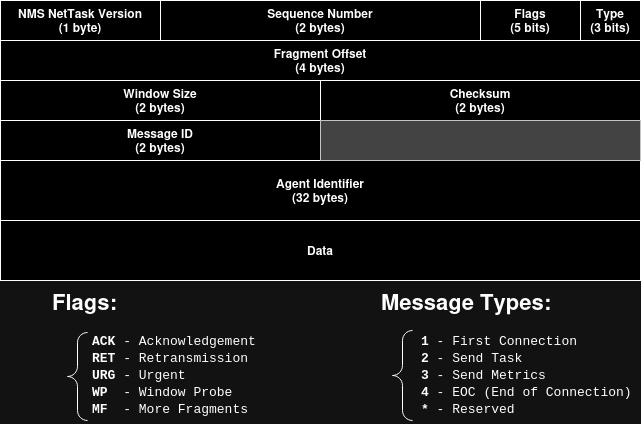
\includegraphics[width=\textwidth]{img/nettask_header.png}
    \captionof{figure}{Formato do cabeçalho do protocolo \textit{NetTask}}
    \label{fig:nettask_message_format}
\end{minipage}

\begin{itemize}
    \item \textbf{\textit{NMS NetTask Version}} (1 \textit{byte}):  versão do protocolo,
        para a compatibilidade de versões entre o servidor e os agentes;
    \item \textbf{\textit{Sequence Number}}     (2 \textit{bytes}): número de sequência da mensagem,
        para a ordenação de pacotes, deteção de pacotes duplicados e identificação de \textit{acknowledgements};
    \item \textbf{\textit{Flags}}               (5 \textit{bits}):  \textit{flags} de controlo:
        \begin{itemize}
           \item [\textbf{\textit{ACK}}] (1º \textit{bit}): \textit{Acknowledgement}, utilizado para confirmar a receção de pacotes;
           \item [\textbf{\textit{RET}}] (2º \textit{bit}): \textit{Retransmission}, indica que o pacote é uma retransmissão;
           \item [\textbf{\textit{URG}}] (3º \textit{bit}): \textit{Urgent}, indica que a mensagem é urgente;
           \item [\textbf{\textit{WP}} ] (4º \textit{bit}): \textit{Window Probe}, utilizado para controlo de fluxo;
           \item [\textbf{\textit{MF}} ] (5º \textit{bit}): \textit{More Fragments}, para (des)fragmentação de pacotes.
        \end{itemize}
    \item \textbf{\textit{Type}}                (3 \textit{bits}): tipo da mensagem:
        \begin{itemize}
            \item \textbf{\textit{0 - Undefined}}               : mensagem indefinida, utilizada
                para testes ou quando nenhum tipo de mensagem é aplicável,
                por exemplo no envio de \textit{window probes};
            \item \textbf{\textit{1 - First Connection}}        : primeira conexão de um agente ao servidor;
            \item \textbf{\textit{2 - Send Task}}               : envio de tarefas pelo servidor;
            \item \textbf{\textit{3 - Send Metrics}}            : envio de resultados de tarefas pelos agentes;
            \item \textbf{\textit{4 - EOC (End of Connection)}} : terminação de conexões nos dois sentidos;
            \item \textbf{\textit{* - Reserved}}                : reservado para futuras extensões. (códigos de 5 a 7);
        \end{itemize}
    \item \textbf{\textit{Window Size}}        (2 \textit{bytes}): indica o tamanho da janela de receção,
        para controlo de fluxo;
    \item \textbf{\textit{Checksum}}           (2 \textit{bytes}): soma de verificação da mensagem,
        para deteção de erros;
    \item \textbf{\textit{Message Identifier}} (2 \textit{bytes}): identificador da mensagem,
        utilizado para a desfragmentação e ordenação de pacotes;
    \item \textbf{\textit{Agent Identifier}}   (32 \textit{bytes}): identificador do agente,
        podendo este ser do recetor ou do emissor da mensagem;
    \item \textbf{\textit{Data/Payload}}       (n \textit{bytes}): carga útil da mensagem com
        tamanho variável, contendo a informação a ser transmitida nas mensagens do tipo
        \textit{Send Task} e \textit{Send Metrics}.
\end{itemize}

\subsection{Descrição de Funcionalidades}
\label{subsec:nt_desc_funcionalidades}

\textbf{Fragmentação de Pacotes}

A fragmentação de pacotes é efetuada quando a carga útil da mensagem excede o
tamanho máximo permitido, sendo esta dividida em fragmentos de forma a não exceder
este limite. Cada fragmento é encapsulado num pacote \textit{NetTask} com a
\textit{flag MF} ativado, indicando que existem mais fragmentos a serem enviados.
Para permitir a identificação e ordenação dos fragmentos, é atribuído um
\textit{Message Identifier} único a cada mensagem fragmentada.


\textbf{Retransmissão de Pacotes Perdidos}

A retransmissão de pacotes perdidos é efetuada quando o emissor não recebe um
\textit{acknowledgement} de um pacote enviado, após um determinado intervalo de
tempo. O emissor reenvia o pacote com a \textit{flag RET} ativada, indicando que
se trata de uma retransmissão. O recetor, ao receber um pacote com esta \textit{flag},
descarta o pacote se este já tiver sido recebido anteriormente.


\textbf{Deteção de Erros}

A deteção de erros é efetuada através da soma de verificação da mensagem (\textit{Checksum}),
calculada com base no cabeçalho e na carga útil da mensagem. O recetor, ao receber
um pacote, calcula a soma de verificação e compara-a com a recebida. Se a soma de
verificação calculada for diferente da recebida, o pacote é descartado.


\textbf{Ordenação de Pacotes}

A ordenação de pacotes é efetuada com base no \textit{Sequence Number} da mensagem,
permitindo a reordenação de pacotes que chegam fora de ordem. O recetor mantém
um registo dos pacotes recebidos e descarta pacotes duplicados, reordenando os
pacotes recebidos de forma a garantir a entrega integral e ordenada das mensagens.


\textbf{Deteção e Manuseamento de Pacotes Duplicados}

A deteção e manuseamento de pacotes duplicados, tal como na ordenação de pacotes, recorre ao
\textit{Sequence Number} da mensagem. O recetor mantém um registo dos pacotes recebidos para
deteção de pacotes duplicados, descartando pacotes que já tenham sido recebidos anteriormente, e
enviando um \textit{acknowledgement} ao emissor para confirmar a receção do pacote para evitar
retransmissões desnecessárias.

\textbf{Controlo de Fluxo}

O controlo de fluxo é efetuado através do tamanho da janela de receção (\textit{Window Size}),
indicando ao emissor o número de pacotes que o recetor pode receber sem congestionar a ligação.
O emissor ajusta o tamanho da janela de envio com base no tamanho da janela de receção do recetor,
evitando a sobrecarga da ligação e a perda de pacotes. O recetor, ao receber um pacote, envia um
\textit{acknowledgement} com o tamanho da janela de receção atualizado, permitindo ao emissor ajustar
o tamanho da janela de envio.

\textbf{Conpatibilidade de Versões}

A compatibilidade de versões é garantida através do campo \textit{NMS NetTask Version} do cabeçalho
da mensagem, permitindo a identificação da versão do protocolo entre o servidor e os agentes. Se a
versão do protocolo do emissor for diferente da versão do recetor, a mensagem é descartada, evitando
possíveis incompatibilidades e erros.

\subsection{Diagramas de Sequência}

\begin{itemize}
    \item First Connection
    \item End of Connection
    \item Retransmission
    \item Desfragmentação e Ordenação de pacotes
    \item Controlo de Fluxo
    \item Deteção de Erros
    \item Deteção e Manuseamento de Pacotes Duplicados
\end{itemize}

%===============================================================================
% END PROTOCOLOS APLICACIONAIS
%===============================================================================

%===============================================================================
% BEGIN IMPLEMENTAÇÃO
%===============================================================================

\chapter{Implementação}

\section{\textcolor{red}{Estrutura do Projeto?}}

\section{Parâmetros dos Executáveis}

\section{Ficheiro de Configuração}

\section{Bibliotecas Utilizadas}

\textcolor{red}{
    Dúvida: deve-se referir todas as bibliotecas utilizadas no desenvolvimento? \\
    por exemplo: \textit{socket}, \textit{os}, \textit{sys}, \textit{threading}, etc
    Ou apenas as bibliotecas mais relevantes para a solução? \textit{ping3}, \textit{iperf}, etc
}

\section{\textcolor{red}{Detalhes Técnicos? Maybe}}

%===============================================================================
% END IMPLEMENTAÇÃO
%===============================================================================

%===============================================================================
% BEGIN TESTES E RESULTADOS
%===============================================================================

\chapter{Testes e Resultados}

\textcolor{red}{
    Para além da testagem manual contínua ao longo do desenvolvimento, foram
    desenvolvidos testes unitários para as classes e funções mais críticas do
    sistema. Estes testes foram desenvolvidos com recurso à biblioteca
    \textit{unittest} do Python.
}

%===============================================================================
% END TESTES E RESULTADOS
%===============================================================================

%===============================================================================
% BEGIN CONCLUSÕES E TRABALHO FUTURO
%===============================================================================

\chapter{Conclusões e Trabalho Futuro}

%===============================================================================
% END CONCLUSÕES E TRABALHO FUTURO
%===============================================================================

%===============================================================================
% BEGIN REFERÊNCIAS
%===============================================================================

%% Change biblibography name from “Bibliografia” to “Referências”
\renewcommand\bibname{Referências}

%% https://www.overleaf.com/learn/latex/bibliography_management_with_bibtex
\begin{thebibliography}{9}

\bibitem{DatabaseSystems}
Connolly, T., \& Begg, C. (2015). Database Systems: Example (6th ed.). Pearson Education. London, UK.

% \bibitem{MySQLManual}
% MySQL 8.0 Reference Manual (2024). \href{https://dev.mysql.com/doc/refman/8.0/en/storage-requirements.html}{MySQL 8.0 Reference Manual: Data Type Storage Requirements}. MySQL, Oracle.

\end{thebibliography}

%% Add bibliografia to index
\addcontentsline{toc}{chapter}{Bibliografia}

%===============================================================================
% END REFERÊNCIAS
%===============================================================================

%===============================================================================
% BEGIN ANEXOS
%===============================================================================

%% \addchap has no numbering but appears in table of contents.
\addchap{Anexos}

\addsec{
    \href{https://google.com/}{\small [I] Exemplo de Anexo}
    \label{anexo:1}
}

%===============================================================================
% END ANEXOS
%===============================================================================

\end{document}
